%%%%%%%%%%%%%%%%%%%%%%%%%%%%%%%%%%%%%%%%%%%%%%
%                insertmeeting
% 1) Title (something creative & funny?)
% 2) Date (MM/DD/YYYY)
% 3) Location (ex. Hagerty High School)
% 4) People/Committees Present 
% 5) Picture 
% 6) Start Time & Stop Time (ex. 12:30AM to 4:30PM)
%%%%%%%%%%%%%%%%%%%%%%%%%%%%%%%%%%%%%%%%%%%%%%
\insertmeeting 
	{Awesome Autonomous} 
	{03/08/22} 
	{Hagerty High School}
	{James, Jensen, Nathan, Ritam}
	{Images/RobotPics/robot.jpg}
	{2:30 - 4:30}
	
\hhscommittee{Software}
\noindent\hfil\rule{\textwidth}{.4pt}\hfil
\subsubsection*{Goals}
\begin{itemize}
    \item Remeasure all of the distances and splines we use in autonomous.

\end{itemize} 

\noindent\hfil\rule{\textwidth}{.4pt}\hfil

\subsubsection*{Accomplishments}
One of the main problems for us at States was autonomous inconsistency. One way we planned to approach this problem was remeasuring all of the distances and recalculating our splines. Even though this step may not be necessary, it would set a good foundation for us to build the rest of the autonomous on. At least knowing that all of the distances we are telling the robot to travel should follow the path we want will help in our debugging, since any issues with missed movement would be caused by an issue in our navigation protocols. 


\begin{figure}[htp]
\centering
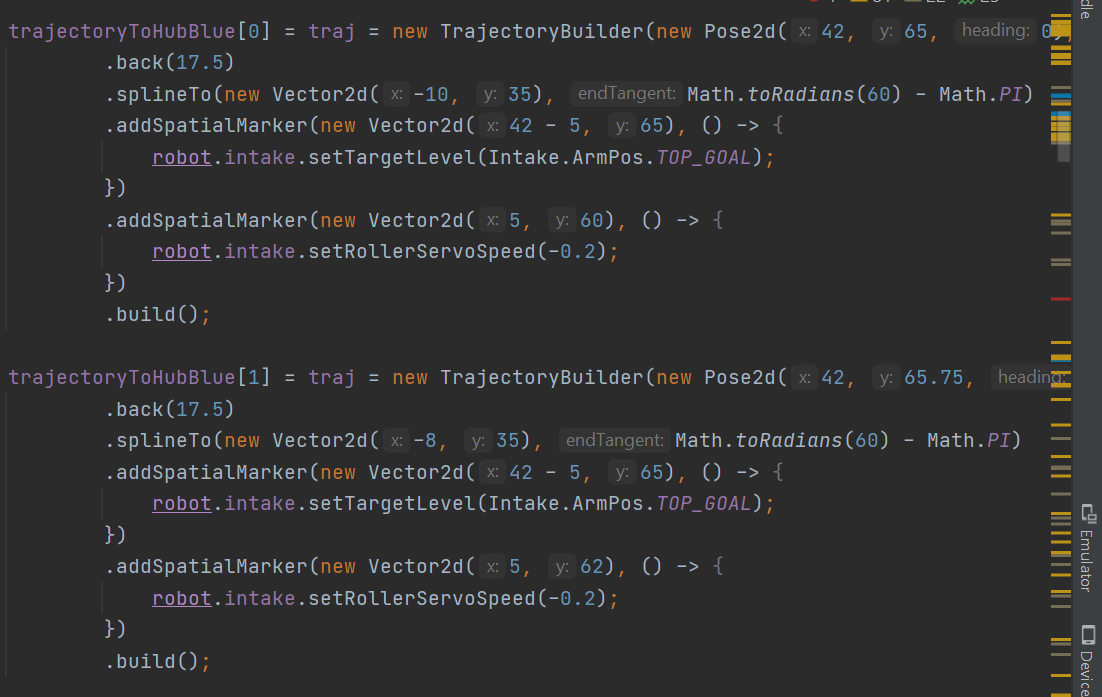
\includegraphics[width=0.95\textwidth, angle=0]{Meetings/March/03-08-22/03-08-22 1.png}
\caption{An example of our remeasured trajectories.}
\label{fig:030822_1}
\end{figure}




\whatsnext{
\begin{itemize}
    \item Prepare for this week's competition.
\end{itemize} 
}

